\documentclass[a4paper,11pt,titlepage]{report}
\pagestyle{plain}

\usepackage[T1]{fontenc}
\usepackage{lmodern}
\usepackage[utf8]{inputenc}
\usepackage[a4paper]{geometry}
\usepackage{draftwatermark}
\usepackage{listings}
\usepackage[toc,page]{appendix}
\usepackage[croatian]{babel}
\usepackage[sc]{mathpazo}
\usepackage{amsmath,amssymb,amsfonts,mathrsfs}
\usepackage{graphicx}
\usepackage[linkcolor=black,colorlinks=true,citecolor=black,filecolor=black]{hyperref}
\usepackage{titlesec}
\usepackage{naslovna}
\usepackage[nomain,acronym,xindy,toc,nonumberlist,automake]{glossaries}
\usepackage{float}
\usepackage[nottoc]{tocbibind}
\usepackage{minted}
\usepackage{CJKutf8}
\usepackage{dingbat}
\usepackage{pmboxdraw}
\usepackage{enumitem}
\makeglossaries
           
\usemintedstyle{emacs}
\setminted{mathescape,
           linenos,
           frame=lines,
           fontsize=\footnotesize,
           baselinestretch=1,
           framesep=2mm,
           breaklines,
           breakautoindent=false,
           breaksymbolleft=\raisebox{0.8ex}{
               \small\reflectbox{\carriagereturn}},
           breaksymbolindentleft=0pt,
           breaksymbolsepleft=0pt,
           breaksymbolright=\small\carriagereturn,
           breaksymbolindentright=0pt,
           breaksymbolsepright=0pt}
           
\setminted[text]{frame=none}
           
%\titleformat{\chapter}
%{\normalfont\huge\sffamily}{\thechapter}{1em}{\textbf}
%
%\titleformat{\section}
%{\normalfont\large\sffamily}{\thesection}{1em}{}
%
%\titleformat{\subsection}
%{\normalfont\large\sffamily}{\thesubsection}{1em}{}
\linespread{1.5}

\renewcommand{\abstractname}{Abstract}
\renewcommand{\contentsname}{Sadržaj}
\renewcommand{\figurename}{Prikaz}
\renewcommand{\tablename}{Tabela}
\renewcommand{\chaptername}{}
\renewcommand{\bibname}{Literatura}
\renewcommand\lstlistlistingname{Indeks listinga}
\renewcommand\listfigurename{Indeks prikaza}
\renewcommand\listtablename{Indeks tabela}
\renewcommand\appendixname{Dodatak}
\renewcommand\appendixpagename{Dodaci}
\renewcommand\appendixtocname{Dodatak}
\renewcommand{\glossaryname}{Pojmovnik}
\renewcommand{\acronymname}{Pojmovnik} 

\newcommand\blankpage{%
    \null
    \thispagestyle{empty}%
    \addtocounter{page}{-1}%
    \newpage}

\SetWatermarkText{}
\SetWatermarkScale{0.8}

\title{Aplikacija za evidentiranje prisustva}
\author{Malik Koljenović, BSc IT}
\thesistype{MSc završni rad}
\mentor{prof. dr. Saša Mrdović}
\department{Odsjek za računarstvo i informatiku}
\faculty{Elektrotehnički fakultet}
\university{Univerzitet u Sarajevu}
\date{Sarajevo, septembar 2018}
\newglossaryentry{LAPP}
{name={LAPP}, description={Logit višekomponentna aplikacijska platforma}}

\newglossaryentry{UI}
{name={UI}, description={Android komponente LAPP platforme}}

\newglossaryentry{LAPI}
{name={LAPI}, description={Logit API, Python serverska aplikacija, komponenta LAPP platforme}}

\newglossaryentry{ATTN}
{name={ATTN}, description={repozitorij potpisanih prisustva spremljen na LAPI}}

\newglossaryentry{CERT}
{name={CERT}, description={javni dio korisničkog kriptografskog ključa}}

\newglossaryentry{SSO}
{name={SSO}, description={\textit{(en. Single Sign On)} - politika autentifikacije korištenjem jedinstvenog repozitorija}}

\newglossaryentry{KEYS}
{name={KEYS}, description={jedinstveni set korisničkih RSA ključeva dužine 2048 bita}}

\newglossaryentry{DEVICE}
{name={DEVICE}, description={korisnički Android uređaj}}

\newglossaryentry{SPIM}
{name={SPIM}, description={\textit{(en. SPacetIME)} - lokacijski dokaz (JSON objekat, struktura podatka)}}

\newglossaryentry{HCE}
{name={HCE}, description={\textit{(en. Host card emulation)} softverska arhitektura koja omogućava virtualnu emulacija elektronskog identiteta}}

\newglossaryentry{M}
{name={M}, description={\textit{(en. master)} - Android UI komponenta pokrenuta na uređaju koji bilježi prisustvo}}

\newglossaryentry{S}
{name={S}, description={\textit{(en. slave)} - Android komponenta koja se izvršava u pozadini na uređaju čije se prisustvo bilježi}}

\newglossaryentry{BUMP}
{name={BUMP}, description={približavanje mobilnih uređaja, otvara jednosmjerni komunikacijski kanal u smijeru od slave (S) prema master (M) uređaju}}

\newglossaryentry{ISO14443A}
{name={ISO/IEC 14443 Tip A}, description={standard fizičkog sloja NFC komunikacijskog protokola}}

\newglossaryentry{NFC Forum Tag}
{name={NFC Forum Tag}, description={standardizovani format NFC taga}}

\newglossaryentry{NDEF}
{name={NDEF}, description={vrsta standardizovanog paketa korištena za NFC komunikaciju između uređaja}}

\newglossaryentry{NDEFMSG}
{name={NDEFMSG}, description={NDEF poruka koja sadrži vremensko-lokacijski dokaz potpisan od strane korisnika}}

\begin{document}
	\maketitle
	\blankpage
	\afterpage{\blankpage}
\paragraph*{Abstract}
This thesis addresses the problem of large scale electronic attendance taking in university setting by presenting an Android based attendance taking application, based on immutable and non repudiable location proofs backed by RSA cryptography, utilizing NFC and HCE for ease of use, emulating NFC Forum Tag Type 4 it is also compatible with existing reader infrastructures. It also presents a general overview of the utilized techologies and select implementation details.

\paragraph*{Apstrakt}
Ova teza tretira problem masovnog elektronskog bilježenja prisustva u univerzitetskom okruženju izradom prijedloga aplikacija bazirane na Android platformi korištenjem neizmjenjivih i neporecivih vremensko-lokacijskih dokaza osiguranih korištenjem RSA kriptografije, te NFC i HCE tehnologija u cilju jednostavnosti upotrebe; emulirajući NFC Forum Tag Tip 4 kompatibilna je sa postojećim infrastrukturama čitača. Dat je i opšti pregled korištenih tehnologija i izdvojenih implementacijskih detalja.

\paragraph*{MSC Primary 68P25; Secondary 94A60;}
\paragraph*{Keywords:} NFC - near-field communication, HCE - host card emulation, security, Android, attendance, RSA, cryptography, NDEF, NTAG, geolocation, location proofs
	\tableofcontents
	\listoffigures
	\listoftables
    \glsaddall
	\printglossaries
	\chapter{Uvod}
Prodor digitalnih računara i komunikacijskih tehnologija u sve sfere ljudskog života i djelovanja, te dramatično povećanje broja korisnika interneta u posljednjoj deceniji nametnulo je mnoštvo novih društvenih i tehničkih izazova. Društveni izazovi najbolje su uočljivi kroz višedecenijsku debatu o privatnosti i vlasništvu nad ličnim podacima, samim time zadiru duboko u diskusiju o ljudskim pravima i identitetu sa jedne i često suprostavljenim komercijalnim interesima sa druge strane. Ukoliko se u tom kontekstu posmatra aktuelna EU uredba o zaštiti podataka\cite{gdpr} (\textit{en. GDPR}) postaje jasno da su digitalna tehnologija i komunikacije postale integralni dio društvene i emocionalno-psihološke realnosti\cite{Searle1995}, do te mjere da se digitalni tragovi smatraju dijelom nepovredivog identiteta osobe. Iz navedenog je jasno da se radi o institucionalizaciji jedne potpuno nove društveno-tehnološke paradigme unutar pravnih okvira Europske unije.

\paragraph*{}
Sa tehničke strane, dostignuća na poljima kriptografije, teorije mreža i novih komunikacijskih tehnologija, te njihova široka prihvaćenost otvorila su mogućnosti izrade računarskih sistema spremnih da odgovore na novonastale društvene izazove u okviru opisane nove paradigme. Pomenuti računarski sistemi kao dodatno izvršno okruženje imaju društveno-pravnu realnost te se u tim okvirima izvršavaju masovno, dobrovoljno, distribuirano i interaktivno\cite{Cahill2003} van centralizovanog računarskog izvršnog okruženja u smislu Von Neumannove arhitekture. Opisani sistemi mogu se okarakterisati kao sistemi potpomaganja (\textit{en. assist}), npr. kriptografski računarski sistem u domenu autentifikacije i autorizacija u novoj paradigmi postmatra se kao sistem računarski-potpomognutog povjerenja, ekvivalentno višem nivou apstrakcije.

\paragraph*{}
Registri u kontekstu društvenih institucija su elementarni mehanizam sistema povjerenja, sigurnosne karakteristike takvih institucionalnih registara stoga čine osnov istraživačkog interesa u domenu institucionalne sigurnosi. Napredni elektronski registri izrađeni korištenjem kriptografskih tehnika i savremenih komunikacijskih protokola za prikupljanje i obradu podataka omogućavaju poboljšanje njihovih sigurnosnih osobina, otvarajući nove načine primjene i stvarajući uslove za viši nivo društvenog razvoja i institucionalne efikasnosti, uz to pružaju i adekvatan odgovor na novonastale društvene izazove. Stoga, ukoliko se obezbijede i ispoštuju preduslovi izrade sigurnog sistema\cite{iso2013iso}, evidenciju prisustva u kontekstu naprednog elektronskog registara treba posmatrati i kao vremensko-prostorni dokaz određenog događaja, ovaj rad usmjeren je na izradu jednog takvog sistema računarski-potpomognutog povjerenja u obliku institucionalnog registra elektonske evidencije prisustva.
	\chapter{Postavka problema}
Projektni zadatak ovog završnog rada je izrada aplikacije na Android platformi sa pripadajućom udaljenom komponentom, koje u cjelini treba da omoguće evidentiranje prisustva nastavnim aktivnostima na Elektrotehničkom fakultetu u Sarajevu. U skladu sa zadatim funkcionalnim zahtjevima, a iz razloga olakšanog korištenja i praktičnosti upotrebe neophodno je iskoristiti beskontaktne komunikacijske mogućnosti savremenih mobilnih telefona u vidu NFC komunikacijskog protokola.
\paragraph*{}
Također neophodno je osigurati korisnike aplikacije od mogućih zloupotreba korištenjem dostupnih kriptografskih metoda i tehnologija, te stvoriti neophodne uslove za sticanje povjerenja u širi sistem bilježenja prisustva putem neporecivosti i neizmjenjivosti prethodno unesenih podataka. Poželjna mogućnost je jednostavna integracija sa postojećim sistemima, prvenstveno onim autentifikacijskim i autorizacijskim, te planiranje arhitekture za buduća proširenja u vidu omogućavanja integracije sa infrastrukturnim hardverskim čitačima i TAG karticama.
\paragraph*{}
Potrebno je dokumentovati proces izrade i opisati korištene tehnologije, sa posebnim osvrtom na korištene kriptografske metode i tehnologije, te identifikovati otvorena pitanja na polju elektronskih registara prisustva, mogućnosti i izazove koje oni predstavljaju uz rješenja koja navedena aplikacija nudi u datom kontekstu.
	\chapter{Prijedlog rješenja}
U skladu sa datim zahtjevima predložena je izrada aplikacijske platforme pod nazivom Logit (
\gls{LAPP}), opisane u nastavku, sa detaljnim tehničkim detaljima u narednim poglavljima. Uzimajući u obzir data ograničenja, te funkcionalne i nefunkcionalne zahtjeve određeno je da se korisnička aplikacija izradi na Android platformi sa podrškom za Android API nivo počevši od nivoa 19 (4.4 KitKat), to je najniži nivo koji omogućava korištenja naprednih NFC i kriptografskih funkcionalnosti te osigurava dobru pokrivenost potencijalne korisničke baze sa ukupnom adopcijom od preko 90\% za navedenu ili višu verziju\cite{droidstats}. Za uspješan rad aplikacije neophodno je da korisnički uređaj podržava i NFC funkcionalnosti, prema prognozama analitičke kuće IHS Technology, do 2020. godine svaki treći uređaj imati će podršku za NFC.\cite{nfcforecast}

\section{Logički model rješenja}
Priloženi dijagrami interakcije osnovnih funkcionalnosti Logit platforme i pripadajući opis imaju za cilj stvoriti opštu sliku sistema, te tako olakšati praćenje tehničkog modela rješenja datog u nastavku. Tehnički model opisuje dosta detaljniju sliku funkcioniranja sistema i može služiti kao svojevrstan uvod u kod platforme.

\subsection*{Registracija korisnika}
\begin{figure}[H]
    \centering
    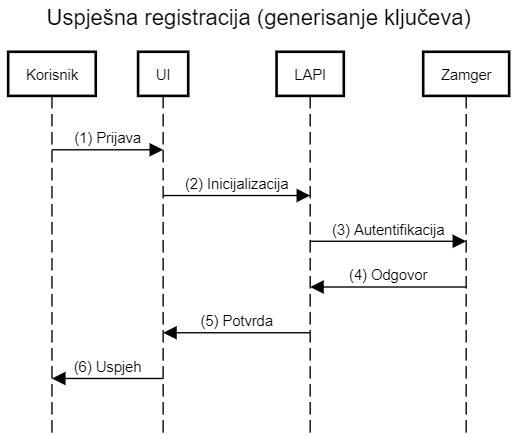
\includegraphics[width=0.7\textwidth]{material/dia/01_registracija}
    \caption{Dijagram interakcije - uspješna registracija i generisanje ključeva}
\end{figure}
\paragraph*{}
Nakon uspješne instalacije aplikacije na korisnički Android uređaj (DEVICE) potrebno je obaviti proces registracije koji se izvršava u dva bitna koraka. Prvi korak sastoji se od unosa već postojećih autentifikacijskih podataka za ZAMGER sistem Elektrotehničkog fakulteta, korisnik se korištenjem datih podataka posredstvom LAPI servisa autentificira na ZAMGER sistemu, bitno je napomenuti da Logit platforma ne sprema korisničku lozinku ZAMGER sistema, navedeni podaci se koriste isključivo za povezivanje postojećeg identiteta i novogenerisanog para korisničkih RSA ključeva (KEYS), što je ujedno i drugi korak u procesu registracije na Logit platformu.

\paragraph*{}
U slučaju uspješnje autentifikacije, korisnika se obavještava o završenoj registraciji te se preusmjerava na glavni ekran za bilježenje prisustva. Generisani javni ključ (CERT) i identifikacioni podaci korisnika spremaju se u LAPI direktorij korisničkih certifikata.

\subsection*{Bilježenje prisustva studenta}
Bilježenje prisustva studenata od strane predmetnog nastavnika izvodi se u Master (M) modu funkcionisanja aplikacije, aplikacija se pri samom pokretanju i nakon uspješno obavljene registracija automatski stavlja u takav mod operacije i u njemu ostaje sve dok je upaljen ekran korisničkog uređaja (DEVICE) i Logit aplikacija (UI) se izvršava u prednjem planu \textit{(en. foreground)}, navedene zahtjeve diktira sama Android platforma.

\begin{figure}[H]
    \centering
    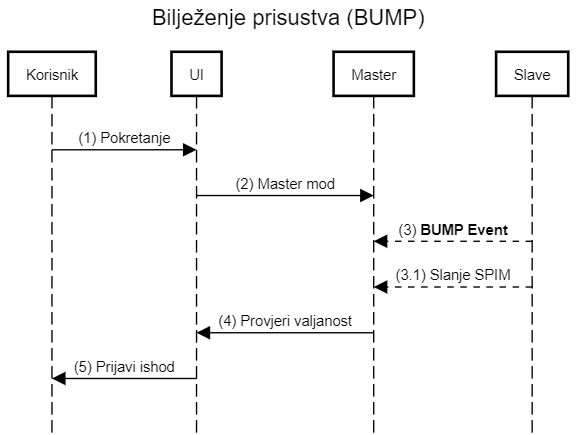
\includegraphics[width=0.7\textwidth]{material/dia/02_bump}
    \caption{Dijagram interakcije - bilježenje prisustva studenata (Master BUMP)}
\end{figure}
\paragraph*{}
Ukoliko su ispunjeni prethodno pobrojani zahtjevi, dovoljno je da student sa podešenom Logit aplikacijom na svom uređaju prinese slave (S) uređaj master (M) uređaju i da njegovo prisustvo bude zabilježeno i prikazano na ekranu M uređaja. Samu interakciju (BUMP) inicira studentski S uređaj. Prilikom ovog BUMP događaja dolazi do razmjene kriptografski potpisanih podataka o vremenu i lokaciji (SPIM) sa S na M, gdje M vrši validaciju primljenih podataka poredeći studentsko vrijeme i lokaciju sa vremenom i lokacijom na M uređaju, gdje se prisustvo odbija ukoliko se ustanovi pokušaj lažiranja podataka.

\subsection*{Prijava prisustva}
\begin{figure}[H]
    \centering
    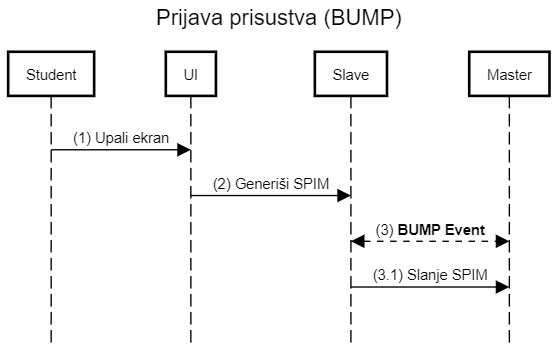
\includegraphics[width=0.7\textwidth]{material/dia/03_prijava}
    \caption{Dijagram interakcije - prijava prisustva studenta (Slave BUMP)}
\end{figure}

\paragraph*{}
Studentski S uređaj i M uređaj nastavnog osoblja podešavaju se na isti način opisan iznad, jedina praktična razlika javlja se prilikom korištenja, gdje je za S uređaj čije se prisustvo bilježi dovoljno upaliti ekran uređaja da bi se mogla ostvariti BUMP interakcija prislanjanjem S na M. Ovo je moguće jer se NFC HCE emulator Logit aplikacije izvršava u pozadini Android sistema.

\subsection*{Pohranjivanje potpisa sesije na LAPI}
Svako bilježenje prisustva unutar Logit Android UI odvija se unutar sesije (SESS) koja se automatski započinje prilikom prvog uspješno zabilježenog prisustva i traje sve dok korisnik ne izvrši pohranu navedene sesije na LAPI servis. Klikom na SYNC dugme prikupljeni podaci šalju se LAPI servisu, provjeravaju se jedinstveni potpisi studenata te potpis ukupne sesije od strane M uređaja, ukoliko se ne pronađu nepravilnosti navedeni podaci se pohranjuju u LAPI repozitorij potpisa, takvi podaci kriptografski su osigurani od naknadne izmjene.

\begin{figure}[H]
    \centering
    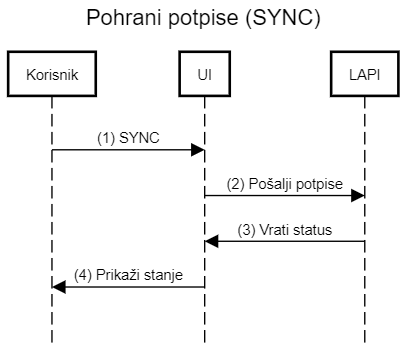
\includegraphics[width=0.6\textwidth]{material/dia/04_sync}
    \caption{Dijagram interakcije - pohranjivanje potpisa na LAPI (SYNC)}
\end{figure}
\paragraph*{}
Potpisi pohranjeni u LAPI repozitoriju mogu dalje biti korišteni u integrisanim aplikacijskim rješenjima koja zahtijevaju ovakvu vrstu podataka pomoću ponuđenog LAPI REST interfejsa, te se mogu smatrati relevantnim i sigurnim dokazom prisustva.

\section{Tehnički model rješenja}
Uvodi se dodatno pojam lokacijskog dokaza\cite{locproof} koji u širem smislu u kontekstu podređenog korisnika (en. slave), obuhvata kriptografski potpisan korisnički identitet, korisnički uređaj, vrijeme i GPS lokacijske podatke korisničkog uređaja. Za svrhu osiguranja jedinstvenosti identiteta i vjerodostojnosti potvrde lokacijskih dokaza odabrano je korištenje RSA asimetrične enkripcije, gdje se pri uspješnoj autentifikaciji generiše jedinstveni set ključeva za korisnički uređaj, privatnom dijelu ključa nije moguće pristupiti izvan aplikacije (SEC1), niti je moguće eksportovati ključ (SEC2), a u određenom vremenskom period može postojati samo jedan valjan set ključeva za jednog korisnika jer se raniji ključevi ne uzimaju u obzir ukoliko postoji noviji set (SEC3), sprječavajući tako replikaciju identiteta na više uređaja.

\paragraph*{}
Pored Android komponente aplikacije (UI) izrađena je i serverska aplikacija u programskom jeziku Python (LAPI), čija je namjena posredovanje u komunikaciji sa autentifikacijskim agentom (ZAMGER), te pohranjivanja i održavanje javnih korisničkih kriptografskih ključeva (CERT) i njihovo povezivanje sa autentifikacijskim podacima korisnika, pored toga služi i kao repozitorij za potpisana prisustva (ATTN). Na ovu komponentu se može gledati kao na integrisani namjenski repozitorij korisničkih certifikata i domenski repozitorij neporecivih i neizmjenjivih lokacijskih dokaza (SPIM).

\paragraph*{}
Budući da na Elektrotehničkom fakultetu u Sarajevu postoji SSO (en. Single-Sign On) politika autentifikacije, u serverskoj komponenti (LAPI) je implementiran autentifikacijski posrednik koji prilikom prvog pokretanja aplikacije prijavljuje korisnika koristeći postojeće pristupne podatke, tom prilikom u slučaju uspješne prijave generiše se i jedinstveni set RSA ključeva dužine 2048 bita (KEYS), koji se pohranjuju na korisničkom uređaju (DEVICE), a javni dio, tj. certifikat (CERT) se pohranjuje i u repozitorij ključeva (LAPI) sa poveznicom na korisnički identitet, kasnije se ti certifikati koriste za provjeru valjanosti potpisa lokacijskih dokaza (SPIM).

\paragraph*{}
Da bi se osigurala jednostavnost korištenja aplikacije odabrana je implementacija HCE emulacijskog načina rada NFC komunikatora koji omogućava korisniku da izvrši komunikaciju sa drugim uređajem bez potrebe da pokreće aplikacijski prozor na svom uređaju, dovoljno je da upali ekran svoj uređaja i prinese ga master (M) uređaju koji prikuplja potpise, u ovom slučaju drugoj instanci Logit aplikacije na kojoj je pokrenuta aktivnost za prikupljanje potpisa (LAPP).

\paragraph*{}
Približavanjem mobilnih uređaja (BUMP) otvara se jednosmjerni komunikacijski kanal u smijeru od slave (S) prema master (M) uređaju korištenjem ISO/IEC 14443 Tip A komunikacijskog protokola pri čemu se emulira NFC Forum Tag tipa 4 i putem NDEF Aplikacije prenosi jedna NDEF poruka (NDEFMSG) koja sadrži vremensko-lokacijski dokaz potpisan od strane korisnika, nadalje u tekstu označen kao SPIM (en. spime)\cite{bruces}.

\paragraph*{}
Po primitku poruke nadređeni uređaj (en. master) koji osluškuje da mu se pridruže podređeni uređaji (en. slave) i ima pokrenutu Logit aplikaciju, tu poruku sprema u lokalni repozitorij potpisa ukoliko ona zadovolja uslove da očitana slave GPS lokacija nije udaljena više od 50 metara od očitane master GPS lokacije (VK1 - validacijski kriterij \#1), te da podešena razlika satova master i slave uređaja nije veća od 300 sekundi (VK2), bez da nad SPIM objektom vrši ikakve izmjene, ukoliko SPIM objekat ne zadovoljava date validacijske kriterije odbija se i ispisuje se odgovarajuća poruka na master ekranu. Moguće je naknadno klikom na validacijsko dugme (ACTVAL) u korisničkom interfejsu izvršiti provjeru svih prikupljenih potpisa tokom jedne sesije (SESS), tom prilikom se, ukoliko postoji mrežna veza; svi potpisi pošalju Logit serveru (LAPI) na provjeru i vraća se stanje valjanosti potpisa za sve proslijeđene SPIM objekte.

\paragraph*{}
Ukoliko master (M) želi da pohrani SPIM objekte iz jedne sesije (SESS) na Logit server (LAPI), klikom na sinhronizacijsko dugme u interfejsu (ACTSYNC), on vrši dodatno potpisivanje svakog SPIM objekta svojom komponentom privatnog ključa (MPRK), tako što potpiše hash (SHA256) vrijednost SPIM objekta (AID) sa dodatim svojim jedinstvenim master korisničkim imenom (MUSER) i jedinstvenim identifikatorom sesije (SID) i dodatno generiše SHA256 vrijednosti tih potvrda (CID), nakon čega objedinjuje sve CID vrijednosti i dodatno ih potpisuje svojim MPRK, sve te vrijednosti šalje Logit server (LAPI) na pohranjivanje, ovakvom procedurom se obezbjeđuje neporecivost i neizmjenjivost SPIM i SESS objekata, jer onemogućava izmjene pojedinačnih SPIM objekata, te brisanje ili dodavanje objekata u finaliziranoj sesiju (SESS) od strane malicioznih aktera bez da naruši integritet SHA256 vrijednosti.

\paragraph*{}
Uzmimajući u obzir bitnost rješenja i visoku vjerovatnoću svakodnevne primjene kod ciljane korisničke grupe, te izazove koje takav slučaj korištenja predstvalja omogućena je i direktna e-mail komunikacija za prijavu grešaka ili slanje prijedloga sa glavnog korisničkog interfejsa (ACTBUG). Kako se radi o slojevitom i kompleksnom softverskom rješenju za više detalja referirati se na izvorni kod priložen u dodatku.

\begin{figure}[H]
    \centering
    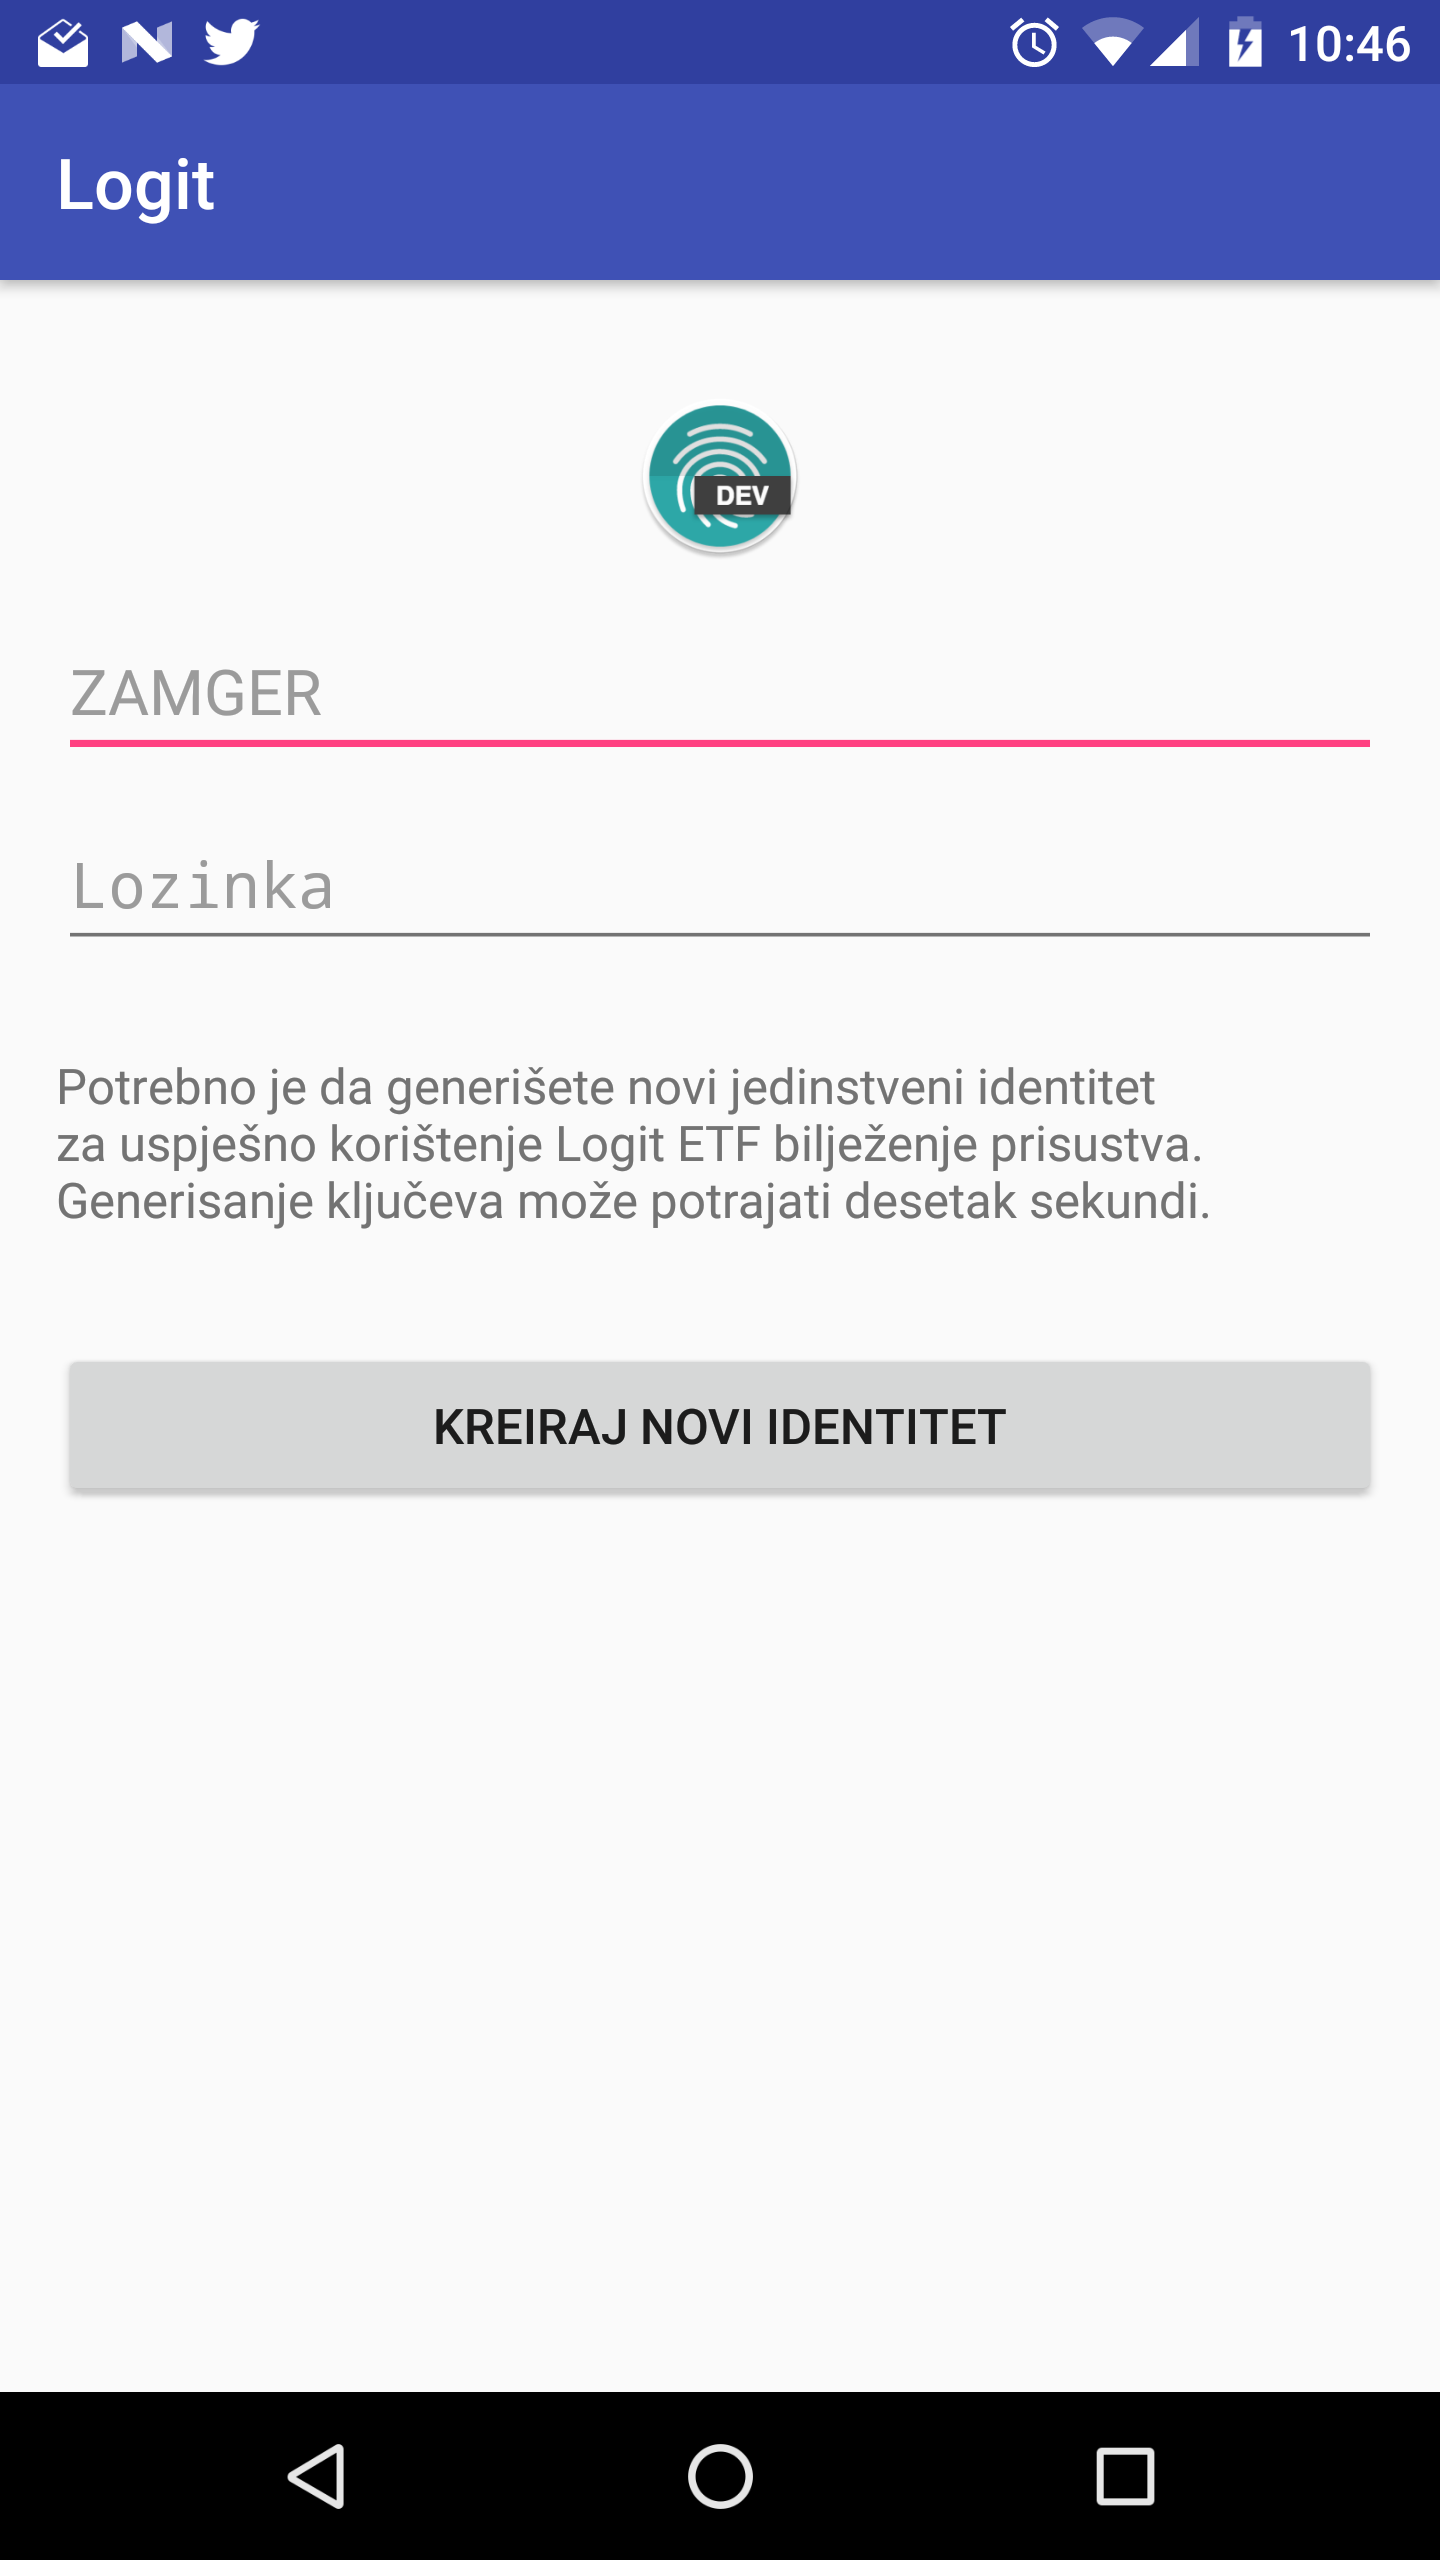
\includegraphics[width=0.45\textwidth]{material/00-login}
    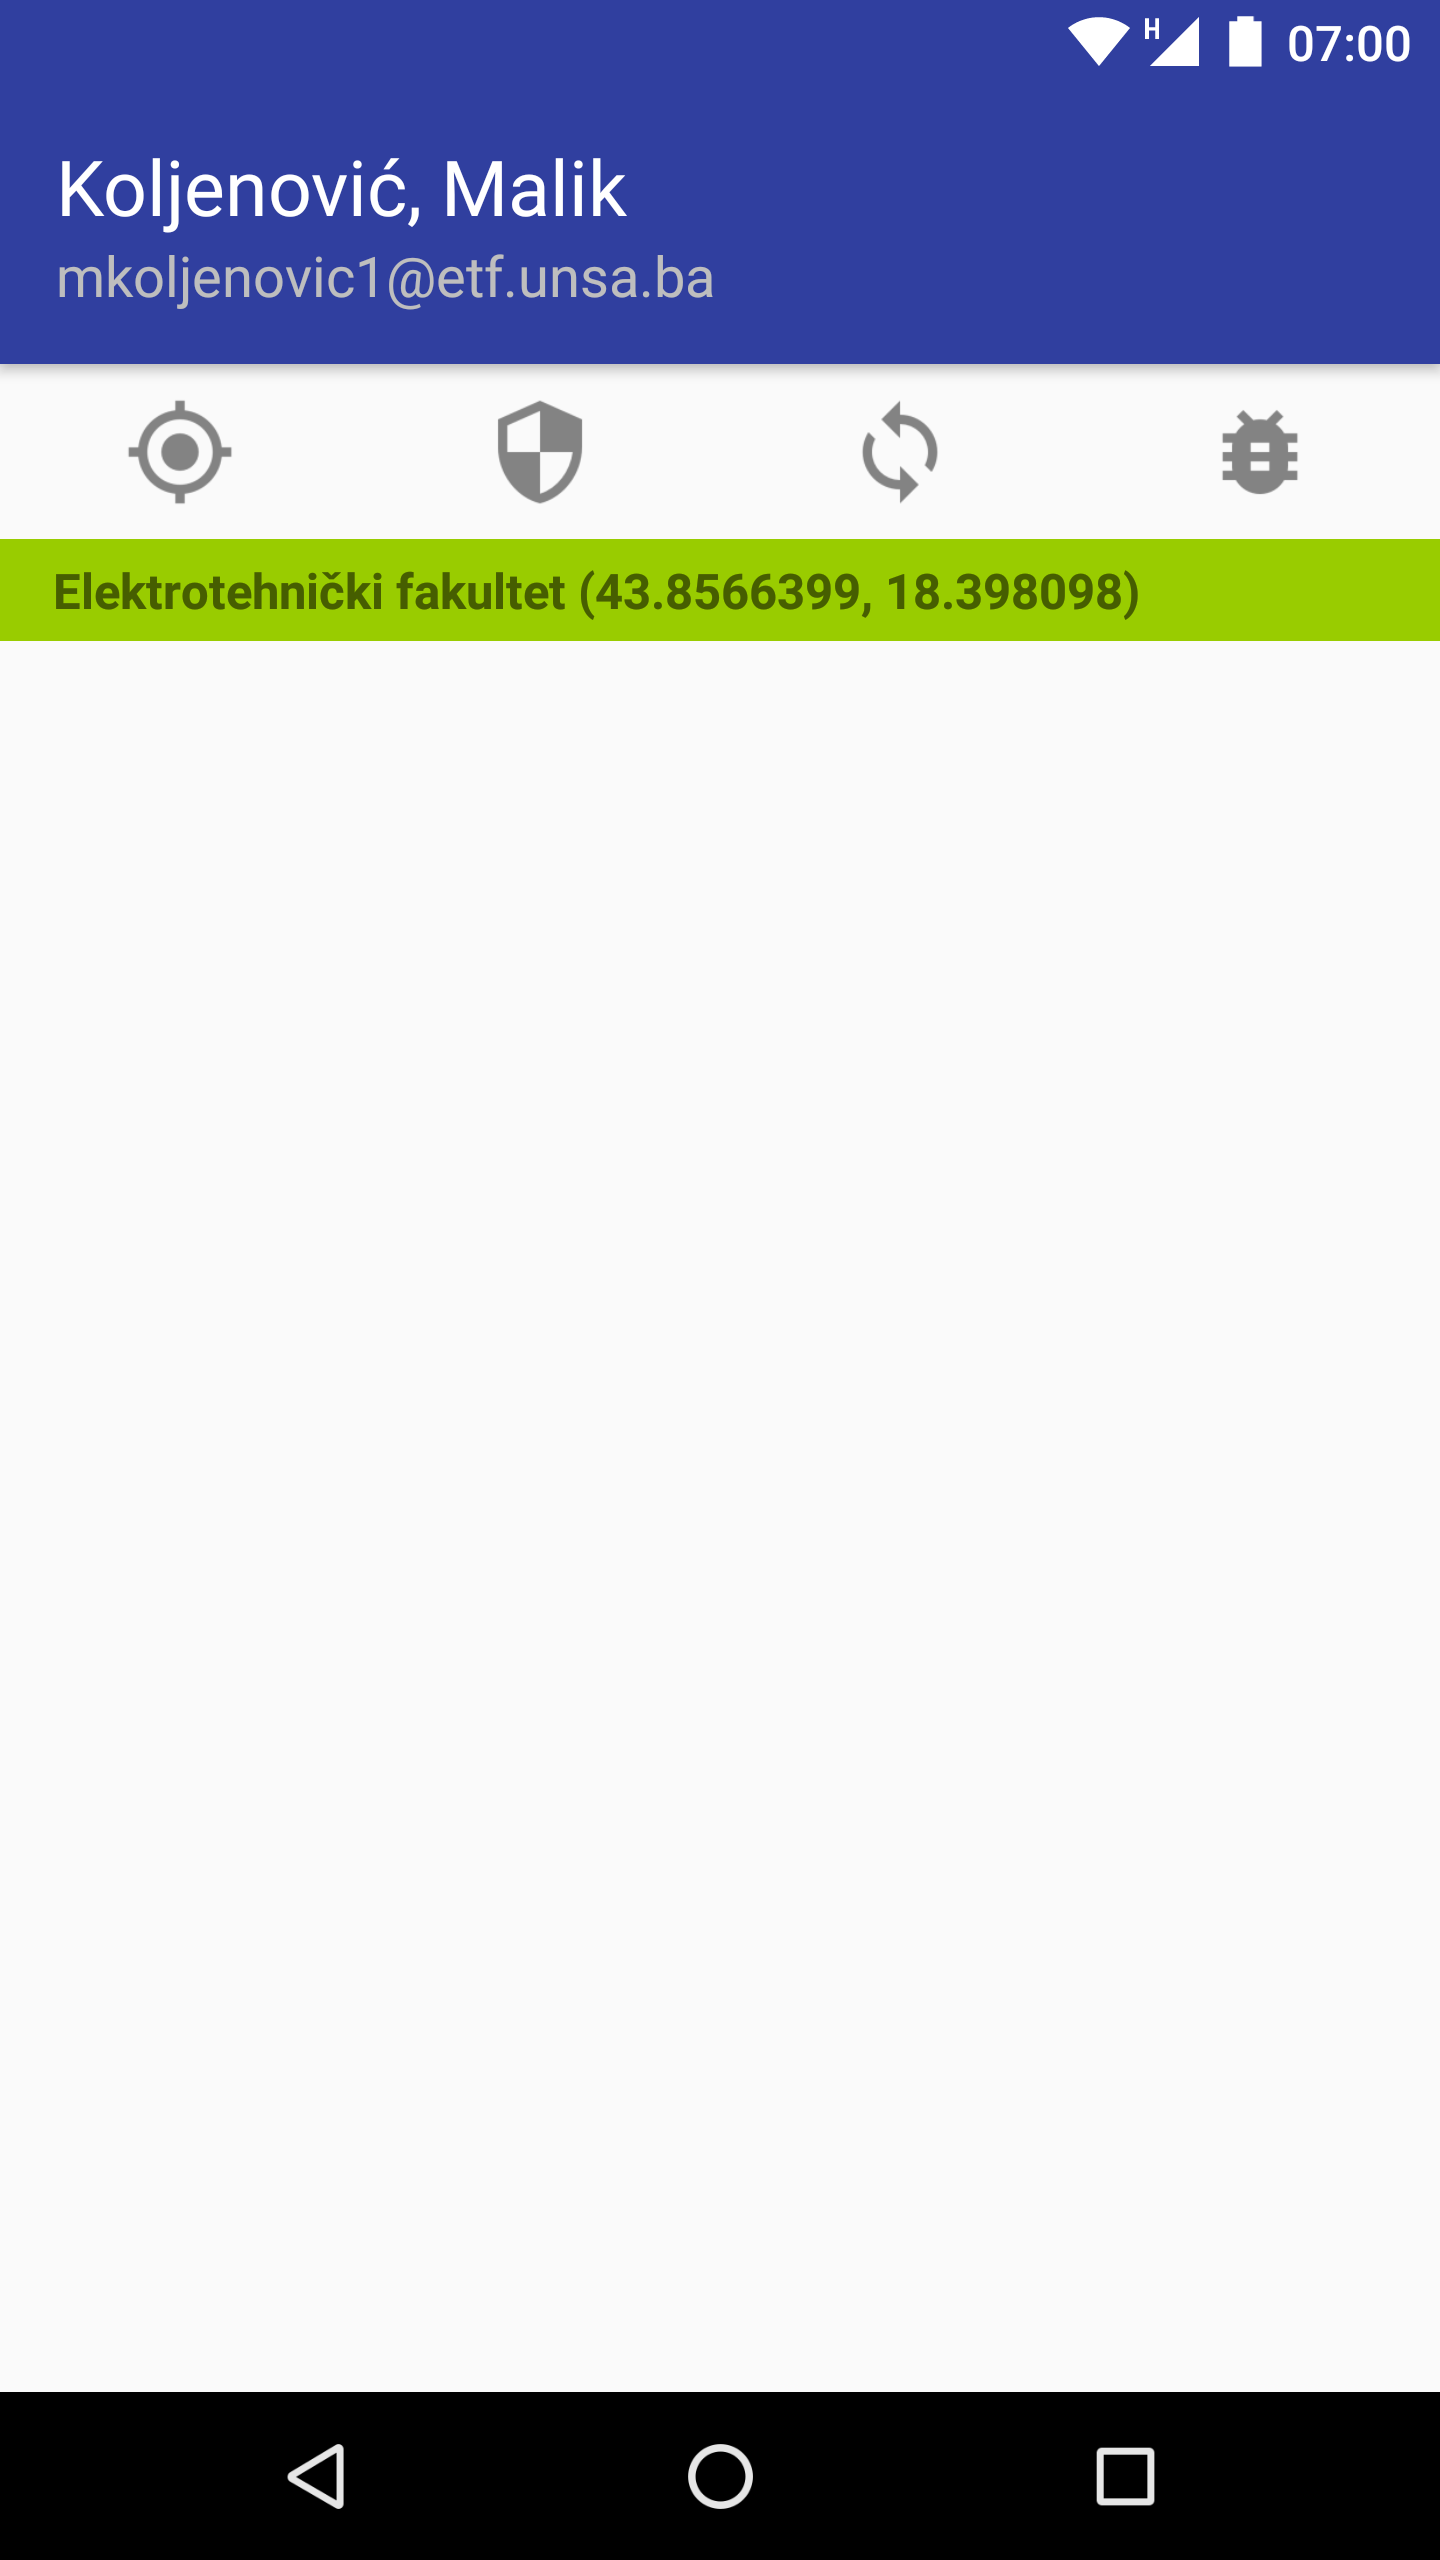
\includegraphics[width=0.45\textwidth]{material/01-attendance}
    \caption{Logit UI Android prikaz korisničkog interfejsa}
\end{figure}
	\chapter{Pregled korištenih tehnologija} \label{chapter:tech}

\section{NFC \textit{(en. near-field communication)}}
NFC skup protokola omogućava uspostavu komunikacijskog kanala između dva uređaja koji se nalaze u neposrednoj blizini jedan drugog (1-4 cm) i razmjenu podataka između njih\cite{NFCProtocol}. Komunikacija se odvija na način da MASTER uređaj osluškuje signal na prijemniku i u slučaju detektovanje SLAVE signala uređaja pošiljaoca, propisanog istim standardom zaprima podatke i vrši obradu nad njima, komunikacija se u većini slučajeva odvija jednosmjerno kratkim standardiziranim porukama (NDEF), no moguće je ostvariti i half-duplex komunikaciju između uređaja, kao i razmjenu nestandardnih poruka, u kojem slučaju se sam korisnik mora pobrinuti za implementaciju kompletnog komunikacijskog protokola. Potpuni detalji implementacija dati su u referencama relevantnih standarda u nastavku tehničkog pregleda, odličnu sintezu detalja i implementacije daju Igoe, Coleman i Jepson\cite{Igoe2014}.
\subsection{NXP NTAG216}
U cilju zadovoljenja postavljenih funkcionalnih zahtjeva bilo je neophodno odabrati NFC Tag platformu koja će odrediti relevantne standarde pohrane binarnih podataka na uređajima kao i pripadajuće komunikacijske protokole, također dodatno su postavljeni zahtjevi ekonomičnosti implementacije i kompatibilnosti sa postojećim čitačima. Uzimajući u obzir nabrojane kriterije odabrana je platforma NTAG216 proizvođača NXP Semiconductors\cite{NTAG216} bazirana na NFC Forum Tag tipu 2 i ISO/IEC14443 Tip A specifikaciji\cite{NFCTag2}\cite{ISO14443}. 

\paragraph*{}
Mogućnosti navedene platforme dostatne su za ispunjenje navedenih funkcionalnih uslova, a pružaju i neke dodatne sigurnosne mehanizme - poput neizmjenjivog jedinstvenog serijskog broja svakog taga (Tag UID) potpisanog kriptografskim ključem proizvođača, navedena funkcionalnost nije implementirana u predstavljenom rješenju jer se bazira na zaštićenoj NXP tehnologiji i nije kompatibilna sa HCE emulacijom, no umnogome može doprinijeti ukupnoj sigurnosti fizičkih Tag čipova u slučaju produkcijske implementacije rješenja. U nastavku je data proizvođačka lista izdvojenih funkcionalnosti NTAG216:

\begin{itemize}[noitemsep]
    \item 7-bajtni UID programiran od strane proizvođača za svaki tag
    \item mogućnost jednokratnog programiranja i zaključavanja taga za dalje izmjene
    \item mogućnost read-only zaključavanja taga
    \item potpis originalnosti baziran na kriptografiji eliptičnih krivih
    \item zaštita memorijskih operacija 32-bitnom lozinkom
\end{itemize}

\paragraph*{}
Proces emulacije taga svodi se na što vjerniju reprezentaciju memorijskog prostora fizičkog uređaja u skadu sa relevantnim standardima, a opcionalno i dodatnih nestandardnih funkcionalnosti u vidu komunikacijskog protokola za korištenje naprednih funkcionalnosti date platforme. Kao minimum neophodan za standardnu komunikaciju NDEF porukama potrebno je emulirati generičko zaglavlje u obliku \textit{CC - capability container} i potpun zapis same NDEF poruke unutar korisničkog memorijskog prostora, potpun prikaz organizacije memorije NTAG216 platforme dat je na slici \ref{fig:ntag_mem}\cite{NTAG216}. Za emulaciju nestandardnih dijelova, poput zaštite čitanja korisničkog memorijskog prostora lozinkom ili emulaciju serijskog broja, za svaku različitu platformu neophodno je implementirati komunikacijski protokol u skladu sa proizvođačkom specifikacijom.

\begin{figure}[H]
    \centering
    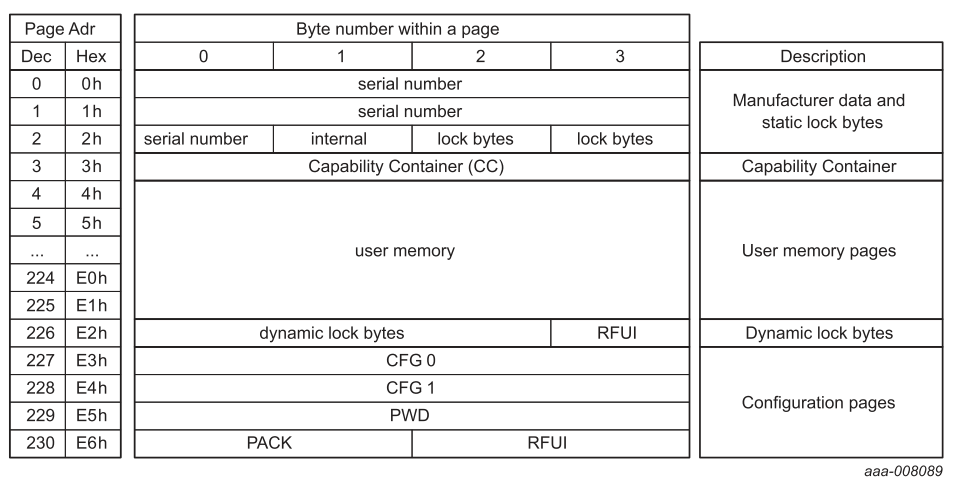
\includegraphics[width=1\textwidth]{material/ntag216-memory}
    \caption{NTAG216 organizacija memorije}
    \label{fig:ntag_mem}
\end{figure}

\subsection{NDEF \textit{(en. NFC Data Exchange Format)}}
NDEF specifikacija definiše \textbf{format enkapsulacije poruke} za razmjenu informacija između dva NFC uređaja. NDEF je lagan binarni format poruke i može se koristiti za enkapsulaciju jednog ili više aplikacijski-definisanih tereta \textit{(en. payload)} raznih vrsta i veličina unutar jedne NDEF poruke. Svaki teret opisan je od strane tipa, dužine i opcionalnog identifikatora. Identifikatori tipa mogu biti URI, MIME media tipovi, ili NFC-specifični tipovi. NDEF je striktno \textbf{format} poruke i ne poznaje pojam konekcije ili logičkog kola.\cite{NDEF}

\paragraph*{}
Neki od ciljeva koje NDEF nastoji da ispuni:
\begin{itemize}[noitemsep]
    \item enkapsulacija dokumenata i binarnih objekata, slika etc.
    \item enkapsulacija podataka nepoznate dužine, npr. stream-a podataka
    \item agregacija srodnih sadržaja unutar jedne poruke
    \item kompaktna enkapsulacija malih datagrama
\end{itemize}

\subsection{HCE \textit{(en. Host card emulation)}}
HCE je metod emuliranja virtuelnog identifikacijskog modula korisnika, u osnovi to je način zaobilaska hardverskih ograničenja (\textit{en. hack, workaround}) koja onemogućavaju direktan pristup SIM (\textit{en. Subscriber Identification Module}) modulu kod mobilnih telefonskih uređaja\cite{elenkov_2012}, ovakvo rješenje vuče korijene iz ekonomske realnosti sektora mobilnih komunikacija i kartičnog plaćanja, koja se najpreciznije može okarakterisati kao oligopol, naime Google je nastojao integrisati SIM karticu unutar Android operativnog sistema u vidu eSE (\textit{en. embedded Secure Element}) korištenjem već postojeće SIM kartice operatera a u svrhu razvoja Google Wallet rješenja, no to nije odgovaralo operaterima i odbili su suradnju, nakon toga Google iznalazi alternativne načine rješenja problema poput HCE\cite{randomoracle_2014}.

\paragraph*{}
HCE na Android OS radi, kako i naziv govori u CE (\textit{en. Card Emulation}) SLAVE modu, gdje se na svaki BUMP sa NFC čitačem odašilju pripremljeni podaci. Podaci koji se pri tome šalju moraju pratiti standard kartice koju žele emulirati i najčešće se vrši prijenos dokumenta ili datagrama unutar jednog ili više NDEF paketa. Logit koristi pristup prijenosa JSON formatiranog SPIM objekta \texttt{plain/text} unutar jednog NDEF paketa. Radi se o konceptu sa mnoštvom implementacijskih detalja, više detalja dostupno je u službenoj dokumentaciji\cite{androidhce_2018}, dok su izvrstan logički prikaz sa primjerima dali Coskun, Oz, Ozdenizci\cite{coskunAndroid}\cite{coskunNFC}, kao i Elenkov\cite{Elenkov2015} u znatno ažurnijem izdanju.

\section{Ostalo}
Dodatno koristi se Android arhitektura za dobavljanje geolokacije\cite{geoa} uz reverzno geokodiranje od strane OpenStreetMap Nominatim projekta\cite{nominatim}. Za potpisivanje i enkripciju korisničkih podataka koristi se RSA\cite{rivest1978method} kriptografija sa 2048 bit ključem. LAPI je Python flask API, kompletan listing koda dostupan je na GitHub u repozitorijima \texttt{koljenovic/logit} i \texttt{koljenovic/logit-node}.
	\chapter{Izdvojeni detalji implementacije}
Detalji izdvojeni u ovom poglavlju ključni su za razumijevanje sigurnosnog modela aplikacije, sa tog aspekta posebno su zanimljiva dva objekta, \texttt{Attendance} i \texttt{Session}, koji u osnovi predstavljaju proširene kriptografski potpisane SPIM i SESS objekte.

\section{Podatkovni i kriptografski primitivi}
\subsection{SPIM paket}
Spim u širem smislu predstavlja vremensko-lokacijski objekat (\textit{en. SPace-tIMe}), koji korištenjem kriptografske obrade poprima karakteristike lokacijskog dokaza. Izvor za formiranje SPIM objekta sastoji se iz korisničkog imena studenta, geografske širine, geografske dužine i trenutnog vremena na studentovom mobilnom uređaju. Ovako komponovan objekat predstavlja implementaciju lokacijskog dokaza u užem smislu i koristi se dalje kao osnovni podatkovni primitiv za dalju kriptografsku obradu.

\inputminted{text}{material/logit_tag.txt}

\paragraph*{}
Navedene vrijednosti stringova korisničkog imena studenta, geografske širine, geografske dužine i trenutnog vremena se lančaju u jedan string izloženim redoslijedom i takav string se potpisuje korištenjem RSA kriptografije, tako potpisan paket u obliku JSON objekta (prikazan u listingu iznad) šalje se na profesorski master uređaj, gdje se dodaju podaci sesije, u vidu jedinstvenog identifikatora sesije (SID), te se potpisano studentsko prisustvo obilježava jedinstvenim heksadecimalnim identifikatorom AID izvedenim iz potpisa prisustva putem SHA256 hash funkcije, navedene vrijednosti, SID i AID se lančaju u jedan binarni string i potpisuju od strane profesora (CONFSIG), naknadno se na iz SHA256 hash vrijednosti CONFSIG profesorskog potpisa formira finalni identifikator potvrde prisustva CID, time se završava kriptografsko osiguravanje valjanosti prisustva u smislu SPIM objekta.

\begin{figure}[H]
    \centering
    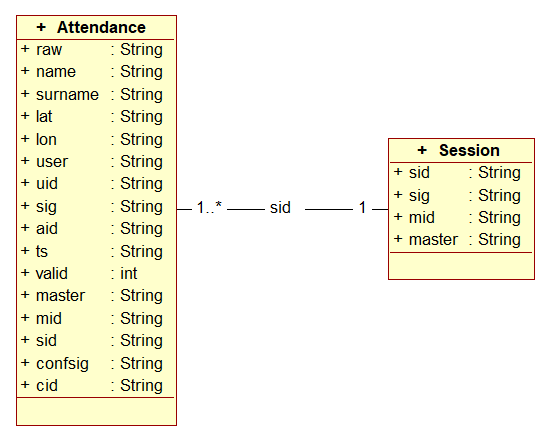
\includegraphics[width=0.6\textwidth]{material/classmodel}
    \caption{Dijagram klasa SPIM i SESS objekata}
\end{figure}
\begin{description}[align=right,labelwidth=2cm,noitemsep]
    \item [raw] serijalizirana string JSON verzija objekta
    \item [name] ime studenta
    \item [surname] prezime studenta
    \item [lat] geografska širina student
    \item [lon] geografska dužina student
    \item [user] ZAMGER korisničko ime studenta
    \item [uid] User ID - SHA2 hex hash javnog ključa studenta
    \item [sig] hex potpis SPIM-a (user:lat:lot:ts)
    \item [aid] Attendance ID - hex SHA2 hash \texttt{sig} potpisa
    \item [ts] vrijeme na studentovom uređaju
    \item [valid] validation cache
    \item [master] ZAMGER korisničko ime profesora
    \item [mid] Master ID - SHA2 hex hash javnog ključa profesora
    \item [sid] Session ID - identifikator profesorove sesije
    \item [confsig] Master Conf. profesorov hex potpis (sid:aid)
    \item [cid] Confirmation ID - SHA2 hex hash confsig-a
\end{description}

\paragraph*{}
Fizički predstavljen opisani SPIM objekat manji je od 1 KB te je pored brzog NFC isl. elektronskog transfera moguće izvršiti prenos alternativnim metodama, kao posebno pogodna čini se QR kod reprezentacija\cite{soon2008qr} i prenos, koja može biti vrlo korisna u slučaju da nijedan od uređaja ne posjeduje NFC modem. Navedeni modus nije implementiran u aplikaciji i dat je kao sugestija zaobilaženja hardverskih ograničenja, primjer QR oblika ranije datog SPIM objekta prikazan je na slici \ref{img:qr}.

\paragraph*{}
Dati QR prikaz je čitljiv ali je vidno uočljiva gustina zapisa koja može predstavljati problem u slučaju lošije kvalitete medija prikaza, u tom slučaju, kompletan SPIM paket moguće je značajno smanjiti zamjenom korištenog RSA kriptosistema za kriptosistem baziran na eliptičnim krivim, budući da su ključevi korišteni u tom slučajnu znatno kraći\cite{atmelecc}, dužina navedenog potpisa bila bi smanjena sa 512 na minimalno 71 bajt\cite{cheneau2009ecc} navedeni pristup nije prihvaćen u okviru ovog rada zbog povećanja kompleksnosti pokaznog sistema, no praktična implementacija moguća je bez većih programskih izmjena.

\begin{figure}[H]
    \centering
    \begin{subfigure}{.5\textwidth}
        \centering
        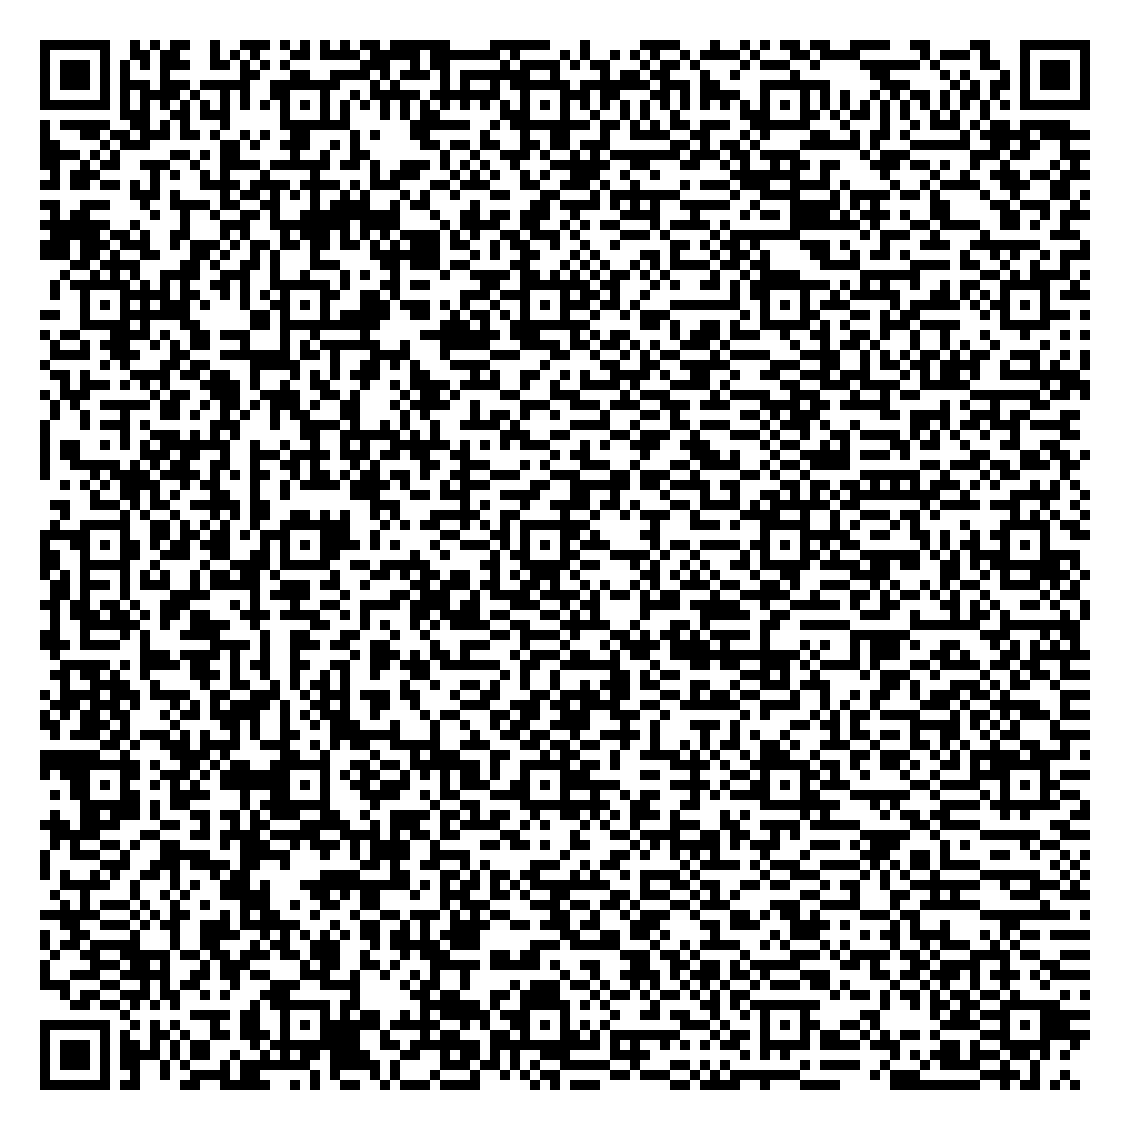
\includegraphics[width=.8\textwidth]{material/logit_qr}
        \caption{oblik korištenjem RSA potpisa}
        \label{img:qr_rsa}
    \end{subfigure}%
    \begin{subfigure}{.5\textwidth}
        \centering
        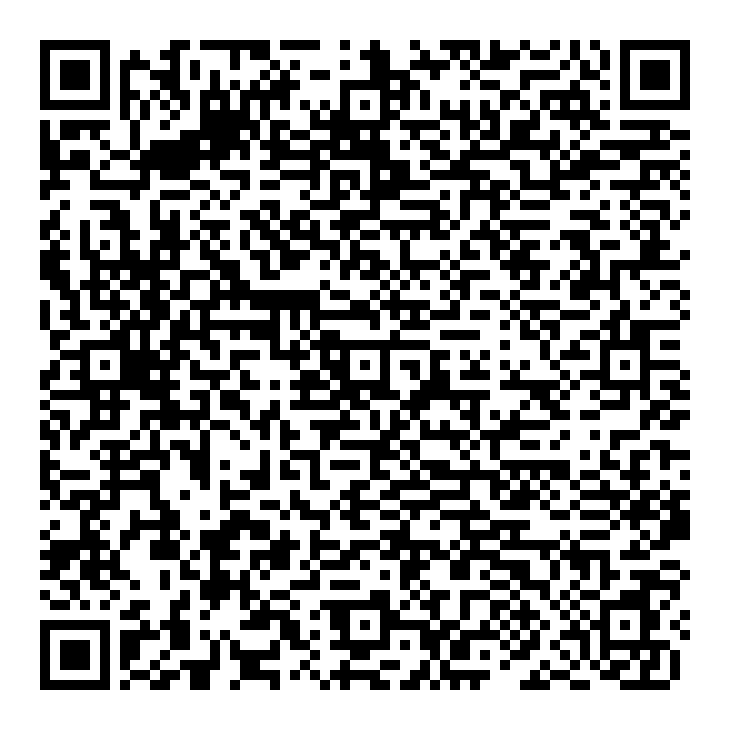
\includegraphics[width=.8\textwidth]{material/logit_qr_ec}
        \caption{oblik korištenjem ECC potpisa}
        \label{img:qr_ecc}
    \end{subfigure}
    \caption{QR oblik SPIM objekta}%
    \label{img:qr}
\end{figure}

\subsection{SESS paket}
Dodatno se za SESS objekat prilikom finaliziranja sesije na LAPI serveru vrši prikupljanje svih CID potpisa koji pripadaju datoj sesiji, te se CID vrijednosti ulančane hronološkim redoslijedom potpisuju LAPI ključem koji se nalazi samo na LAPI hardverskom uređaju, stoga je sigurnost LAPI servera od ključne važnosti za sigurnost ukupnog sistema. Ovako potvrđena sesija ne može biti naknadno mijenjana, lažirana ili porečena izvan LAPI izvršnog okruženja.

\cleardoublepage
\section{Pregled implementacije}
\subsection{MainActivity}
Nakon prvobitnog pokretanja aplikacije a za daljnje uspješno korištenje neophodno je izvršiti autentifikaciju korisnika putem nekog već postoječeg korisničkog repozitorija, te generisati pripadajući virtualizirani sigurni element. Navedene aktivnosti izvršavaju se unutar \texttt{MainActivity} glavnog početnog prozora Logit aplikacije, prikaz relevantnog dijela koda za generisanje virtualiziranog sigurnog elementa dat je u listingu ispod.

\begin{minted}{python}
    KeyPairGenerator kpg = KeyPairGenerator.getInstance(
            "RSA", "AndroidKeyStore");
    Calendar start = Calendar.getInstance();
    Calendar end = Calendar.getInstance();
    end.add(Calendar.YEAR, 1);

    KeyPairGeneratorSpec spec =
            new KeyPairGeneratorSpec.Builder(this).setAlias("etf_logit_" + ts)
                    .setKeySize(2048)
                    .setSubject(new X500Principal("CN=users.etf.ba"))
                    .setSerialNumber(BigInteger.valueOf(tsLong))
                    .setStartDate(start.getTime()).setEndDate(end.getTime()).build();

    kpg.initialize(spec);

    KeyPair kp = kpg.generateKeyPair();

    KeyStore ks = KeyStore.getInstance("AndroidKeyStore");
    ks.load(null);
\end{minted}

\paragraph*{}
Sigurnosni element generisan kao u primjeru iznad dalje se pohranjuje na korisničkom uređaju, gdje privatni dio nikada ne napušta uređaj i dostupan je isključivo Logit aplikaciji putem Android KeyStore providera. Javni dio se koristi kao dio identifikatora korisnika, te se dodatno pohranjuje i na Logit API korisnički repozitorij za potrebe identifikacije i verifikacije potpisa lokacijskog paketa.

\subsection{LogitAPDUService}
Ekstenzija Androidovog native interfejsa \texttt{HostApduService} koji za instaliranu aplikaciju sa \texttt{android.permission.BIND\_NFC\_SERVICE} permisijom vrši pokretanje HCE emulatora prilikom svakog starta operativnog sistema, emulator se u ovom slučaju ponaša kao generički NFC NTAG sa korisnički programiranom memorijom u obliku NDEF poruke koja prenosi jedinstveni potpisan studentski lokacijski dokaz. Navedena servisna komponenta aplikacije aktivna je svaki put dok je i ekran uređaja aktivan ili dok korisnik sam ne zaustavi pripadajući servis. Navedene funkcionalnosti postižu se uključivanjem dijela koda datog u nastavku unutar \texttt{<application>} direktive manifest fajla.

\begin{minted}{python}
    <service
        android:name=".LogitApduService"
        android:permission="android.permission.BIND_NFC_SERVICE">
        <intent-filter>
            <action android:name="android.nfc.cardemulation.action.HOST_APDU_SERVICE" />

            <category android:name="android.intent.category.DEFAULT" />
        </intent-filter>

        <meta-data
            android:name="android.nfc.cardemulation.host_apdu_service"
            android:resource="@xml/apduservice" />
    </service>
\end{minted}

\paragraph*{}
Nadalje \texttt{LogitAPDUService} sadrži logiku za ispravno konstruisanje i formatiranje NDEF paketa\cite{tindef} lokacijskog dokaza i njegovo potpisivanje, te ostalu neophodnu kriptografsku obradu. U nastavku će biti dat prikaz kompletnog servisa sa komentarima relevantnih dijelova.

\begin{minted}{python}
    final static int APDU_INS = 1;
    final static int APDU_P1 = 2;
    final static int APDU_P2 = 3;
    final static int APDU_SELECT_LC = 4;
    final static int APDU_READ_LE = 4;
    final static int FILEID_CC = 0xe103;
    final static int FILEID_NDEF = 0xe104;
    final static byte INS_SELECT = (byte) 0xa4;
    final static byte INS_READ = (byte) 0xb0;
    final static byte INS_UPDATE = (byte) 0xd6;
    final static byte P1_SELECT_BY_NAME = (byte) 0x04;
    final static byte P1_SELECT_BY_ID = (byte) 0x00;
    final static int DATA_OFFSET = 5;

    final static byte[] DATA_SELECT_NDEF = {(byte) 0xd2, (byte) 0x76, (byte) 0x00, (byte) 0x00, (byte) 0x85, (byte) 0x01, (byte) 0x01};
    final static byte[] RET_COMPLETE = {(byte) 0x90, (byte) 0x00};
    final static byte[] RET_NONDEF = {(byte) 0x6a, (byte) 0x82};
    final static byte[] FILE_CC = {
            (byte) 0x00, (byte) 0x0f,       // CCLEN - CC container size
            (byte) 0x20,                    // Mapping version
            (byte) 0x04, (byte) 0xff,       // MLe - max. read size
            (byte) 0x08, (byte) 0xff,       // MLc - max. update size

            // TLV Block (NDEF File Control)
            (byte) 0x04,                    // Tag - Block type
            (byte) 0x06,                    // Length
            (byte) 0xe1, (byte) 0x04,       // File identifier
            (byte) 0x04, (byte) 0xff,       // Max. NDEF file size
            (byte) 0x00,                    // R permission
            (byte) 0x00,                    // W permission
    };
\end{minted}

\paragraph*{}
Deklariše konstantne vrijednosti brojnih dijelova neophodnih za kontrukciju standardne NDEF poruke, između ostalog capability fajl koji predstavlja svojevrsno zaglavlje NDEF paketa.

\paragraph*{}
Metoda generateSignature instancira lokacijske servise i vrši konstukciju paketa lokacijskog dokaza kao i kriptografskih primitiva neophodnih za potpisivanje istog. Za konstrukciju lokacijskog dokaza neophodno je pribaviti trenutno vrijeme uređaja, to je prikazano u narednom dijelu koda.

\begin{minted}{python}
    Long tsLong = System.currentTimeMillis() / 1000;
    String ts = tsLong.toString();
    byte[] signature;
\end{minted}

\paragraph*{}
Nakon toga vršti se instanciranje i učitavanja Android KeyStore objekta koji sadrži korisnički par ključeva neophodnih za potpisivanje lokacijskog paketa.

\begin{minted}{python}
    KeyStore ks = KeyStore.getInstance("AndroidKeyStore");
    ks.load(null);
    KeyStore.ProtectionParameter pp = new KeyStore.PasswordProtection(null);
\end{minted}

\paragraph*{}
Nadalje iz \texttt{KeyStore} objekta učitava se najažurniji virtualizirani sigurnosni element.

\begin{minted}{python}
    Enumeration<String> aliases = ks.aliases();
    String alias = aliases.nextElement();
    Entry entry = ks.getEntry(alias, pp);
\end{minted}

\paragraph*{}
Zbog potrebe za što kompaktnijim prenosom podataka za sve vrijednosti gdje je to moguće generišu se hash preslikavanja koja se kasnije koriste za verifikaciju i pohranjivanje. Za potrebe generisanja hash vrijednosti instancirase SHA-256 \texttt{MessageDigest} objekat.

\begin{minted}{python}
    MessageDigest md = MessageDigest.getInstance("SHA-256");
\end{minted}

\paragraph*{}
Iz virtualiziranog sigurnog elementa dalje učitavamo korisnički certifikat sa javnim ključem, te za potrebe verifikacije identiteta heksadecimalnu reprezentaciju njegove hash vrijednosti pripremamo za uključenje u paket lokacijskog dokaza.

\begin{minted}{python}
    Certificate c = ks.getCertificate(alias);
    byte [] pubKey = c.getPublicKey().getEncoded();
    md.update(pubKey, 0, pubKey.length);
    byte [] pubKeyHash = md.digest();
    String pubKeyHashString = LogitApplication.toHext(pubKeyHash);
\end{minted}

\paragraph*{}
Zatim iz virtualiziranog sigurnog elementa korištenjem korisničkog privatnog ključa pripremamo objekat koji vrši potpisivanje lokacijskog paketa.

\begin{minted}{python}
    Signature s = Signature.getInstance("SHA256withRSA");
    s.initSign(((PrivateKeyEntry) entry).getPrivateKey());
    SharedPreferences userData = getSharedPreferences("UserData", 0);
\end{minted}

\paragraph*{}
Dio lokacijskog paketa koji je pokriven korisničkim digitalnim potpisom sadrži korisničko ime, lokacijske parametre geografske dužine i širine, te vrijeme uređaja u trenutku kreiranja digitalnog potpisa.

\begin{minted}{python}
    String sigPkg = userData.getString("user", "unknown") +
            ":" + location.getLatitude() +
            ":" + location.getLongitude() +
            ":" + ts;
\end{minted}

\paragraph*{}
Takav paket se potpisuje i bilježi se njegova SHA-256 preslikana vrijednost za potrebe verifikacije.

\begin{minted}{python}
    s.update(sigPkg.getBytes("UTF-8"));
    signature = s.sign();
\end{minted}

\paragraph*{}
Osnovni potpisani lokacijski paket se proširuje vrijednostima generisanih SHA-256 preslikavanja i osnovnim korisničkim podacima, te se prosljeđuje metodi createMessage koja formira standardizovan NDEF paket, takav spreman NDEF paket stavlja se na raspolaganje komponenti za prenos putem NFC protokola.

\begin{minted}{python}
    msg = "{\"lat\":\"" + location.getLatitude() +
            "\", \"lon\":\"" + location.getLongitude() +
            "\", \"ts\":\"" + ts +
            "\", \"sig\":\"" + LogitApplication.toHext(signature) +
            "\", \"uid\":\"" + pubKeyHashString +
            "\", \"name\":\"" + LogitApplication.toHext(userData.getString("name", "unknown").getBytes("UTF-8")) +
            "\", \"surname\":\"" + LogitApplication.toHext(userData.getString("surname", "unknown").getBytes("UTF-8")) +
            "\", \"user\":\"" + userData.getString("user", "unknown") + "\"}";

    NdefMessage ndef = createMessage(msg.getBytes("UTF-8"));
    byte[] ndefarray = ndef.toByteArray();

    mNdefFile = new byte[ndefarray.length + 2];

    mNdefFile[0] = (byte) ((ndefarray.length & 0xff00) >> 8);
    mNdefFile[1] = (byte) (ndefarray.length & 0x00ff);

    System.arraycopy(ndefarray, 0, mNdefFile, 2, ndefarray.length);

    logitApp.setMessage(mNdefFile);
\end{minted}

\subsection{processCommandApdu}
Budući da se u prikazanom slučaju vrši emulacija pasivnog NTAG uređaja, APDU servis se izvršava u slave modu i zaprima instukcije od strane master uređaja, neophodno je implementirati parser petlju i logiku za komunikaciju sa master uređajem, unutar koje se vrši prepoznavanje zadatih instrukcija i priprema adekvatan odgovor, navedena logika implementirana je unutar \texttt{processCommandApdu} metode. Kompletna logika emulacije tag uređaja svodi se na prosljeđivanje adekvatnog zaglavlja taga i READ FROM TO binarnog protokola za čitanje memorije koju šalje master, stoga glavninu navedene metode čini jedna switch petlja koja u skladu sa zadatom komandom vraća zaglavlje ili raspon bita emuliranog taga, u ovom slučaju sadržaj koji se emulira je prošireni lokacijski paket iznad. Detalje opisane metode možete pogledati u prilogu koda u dodatku.

\subsection{AttendanceActivity}
Za ostvarivanje pune funkcionalnosti aplikacije neophodna je bila implementacija master moda za prikupljanje i obradu NDEF paketa, u ovom slučaju korisničkih potpisa, enkapsuliranih u obliku potpisanog lokacijskog paketa. \texttt{AttendanceActivity} vrši navedenu funkcionalnost te dodatno vrši provjeru valjanosti potpisa i podataka korisničkih lokacijskih paketa. Verifikacija korisničkih lokacijskih paketa vrši se tako što se korisnički slave podaci o vremenu i lokaciji porede sa podacima o vremenu i lokaciji master uređaja, time se osigurava zaštita od napada lažiranja podataka, te bi za takvu vrstu prevare bila neophodna koluzija dva aktera suprostavljenih interesa, što znatno umanjuje vjerovatnoću takvih napada. Moguće je podesiti vrijednosti dozvoljenih odstupanja verifikacijskih parametara izmjenom koda za tu namjenu datog u nastavku.

\begin{minted}{python}
    final long timediff = System.currentTimeMillis() / 1000 - Long.parseLong(tmpAttn.getTs());
    final Location userLocation = new Location("MOCK");
    userLocation.setLatitude(Double.valueOf(tmpAttn.getLat()));
    userLocation.setLongitude(Double.valueOf(tmpAttn.getLon()));
    if (Build.VERSION.SDK_INT >= 23
            && ContextCompat.checkSelfPermission(that, android.Manifest.permission.ACCESS_FINE_LOCATION ) == PackageManager.PERMISSION_GRANTED
            && ContextCompat.checkSelfPermission(that, android.Manifest.permission.ACCESS_COARSE_LOCATION) == PackageManager.PERMISSION_GRANTED
            || Build.VERSION.SDK_INT < 23) {
        FusedLocationProviderClient mFusedLocatiionClient = LocationServices.getFusedLocationProviderClient(that);
        mFusedLocatiionClient.getLastLocation().addOnSuccessListener(new OnSuccessListener<Location>() {
            @Override
            public void onSuccess(Location location) {
                Float locdiff = userLocation.distanceTo(location);
                if (Math.abs(timediff) < 300) {
                    if (locdiff < 100) {
                        // Lokacija i vrijeme SLAVE uređaja su VALIDNI
                    } else {
                        Toast.makeText(that, "Greška: lokacije udaljene " + locdiff.intValue() + " metara.", Toast.LENGTH_LONG).show();
                    }
                } else {
                    Toast.makeText(that, "Greška: vrijeme nije tačno ili je TAG zastario.", Toast.LENGTH_LONG).show();
                }
\end{minted}

\paragraph*{}
Da bi se izbjegla obaveza reimplementiranja NDEF protokola za podatke primljene putem NFC podatkovnog interfejsa Android nudi predefinisani intent filter za direktnu manipulaciju NDEF poruka, te je za njegovo korištenje potrebno dodati ispod prikazani kod unutar manifest fajla Android aplikacije. Korištenjem ovog filtera programer kao rezultat uspješnog NFC prenosa dobija standardizovanu NDEF poruku spremnu za obradu. Ovaj interfejs se koristi unutar \texttt{AttendanceActivity}.

\begin{minted}{python}
<intent-filter>
    <action android:name="android.nfc.action.NDEF_DISCOVERED" />

    <category android:name="android.intent.category.DEFAULT" />

    <data android:mimeType="application/octet-stream" />
</intent-filter>
\end{minted}

\paragraph*{}
Ostatak koda unutar \texttt{AttendanceActivity} klase koristi se za prikaz i obradu elemenata korisničkog interfejsa master moda za prikupljanje korisničkih potpisa.
	\chapter{Zaključak}
Aplikacija izrađena u okviru ovog rada zadovoljava zahtjeve navedene u postavci zadatka i pripadajućem opisu. Korištene su savremene kriptografske metode za implementaciju sigurnosno osjetljivih funkcionalnosti i osigurano je stabilno okruženje za neometano funkcionisanje aplikacije, dodatno je prema zahtjevima uspješno realiziran NFC komunikacijski interfejs između studentskih i instruktorskih mobilnih uređaja. U cilju lakšeg skaliranja težilo se je što više koristiti standardizovane tehnologije, posebno kada je u pitanju NFC, gdje je dodatno implementirana emulacija NTAG vrste taga kao NDEF medija, time je omogućeno da se sistem u budućnosti prilagodi stacionarnim NFC čitačima i korištenju samostalnih NFC tagova.

\paragraph*{}
Pokušana je pilot primjena sistema u saradnji sa nastavnim osobljem na predmetu "Tehnologije sigurnosti" u školskoj godini 2017/18. kojom prilikom je sačinjen spisak studenata i izvršene pripreme sistema. Navedena pilot primjena okončana je neuspješno zbog otvorenih sigurnosnih pitanja u integraciji sa postojećim sistemima, nedostatka resursa i nepostojanja pokusnog sistema pogodnog za projekte u ranoj fazi testiranja, stoga u cilju povećanja inovativnosti i razvoja novih usluga preporučuje se izrada pokusnih \textit{(en. staging)} sistema odvojenih od produkcijskog u okviru Elektrotehničkog fakulteta u Sarajevu.

\paragraph*{}
Tokom pripreme pilot primjene identifikovano je da značajan broj studenata ne posjeduje NFC omogućene mobilne uređaje, te su za njihove potrebe izrađene NTAG216 NFC token naljepnice, no primjena navedenih tokena uvjetovana je dodatnim istraživanjem i doradom Logit sistema za rad sa NTAG216 da bi osigurao isti ili viši nivo sigurnosnih garancija od onog koje pruža Android izvršno okruženje. Kao dodatna smjernica u istraživanju dat je prijedlog korištenja QR kodova za namjenu supstitucije u slučajevima nepostojanja tehničkih predispozicija za upotrebu sistema na strani korisnika, navedena tehnologija može dati dobre rezultate u praktičnoj primjeni i zavređuje dalji istraživački tretman.

\paragraph*{}
Krajnja težnja Logit rješenja je obuhvatanje cjelokupnog sistema autentifikacije i modeliranje relacija povjerenja u materijalnopravnom okruženju, kroz izradu proširive bazne platforme koja može obuhvatiti digitalizaciju mnoštva svakodnevnih administrativnih zadataka jedne institucije, sa tim ciljem daljnje istraživačke napore zavređuje usmjeriti ka razvoju stabilne PKI infrastrukture, kao i digitalizaciji vjerodostojnih institucionalnih registara poput registra ispita sa ciljem digitalizacije studentskog indeksa i srodnih dokumenata.
	\begin{appendices}
		\chapter{Funkcionalni opis Logit rješenja} \label{ch:man}
\begin{enumerate}
    \item \textbf{Uspostavite internet konekciju} prema uputama vašeg nastavnika.
    \begin{enumerate}
        \item potrebno je da na mreži bude dostupna Logit serverska aplikacija i certifikacijski repozitorij za uspješnu prijavu i korištenje, dostupnost možete provjeriti posjetom na \url{https://logit.mine.nu:5000}
    \end{enumerate}
    \item \textbf{Uključite lokacijske usluge} vašeg Android mobilnog uređaja.
    \begin{enumerate}
        \item detaljno uputstvo možete pronaći na \url{https://support.google.com/accounts/answer/3467281?hl=hr}
    \end{enumerate}
    \item \textbf{Omogućite NFC komunikaciju} na vašem Android mobilnom uređaju i \textbf{isključite Android Beam} uslugu za optimalan rad aplikacije.
    \begin{enumerate}
        \item \texttt{Settings > NFC > Enable}
        \item \texttt{Settings > NFC > Android Beam > Disable}
        \item više detalja za navedene postavke pročitajte na \url{https://support.google.com/nexus/answer/2781895?hl=hr}
    \end{enumerate}
    \item Ukoliko niste, \textbf{omogućite sigurnosnu funkcionalnost zaključavanja vašeg ekrana}
    \begin{enumerate}
        \item Android OS nudi usluge integrisane sigurnosti mobilnih uređaja, te je Keystore funkcionalnost sigurnog pohranjivanja privatnih ključeva usko vezana za ostale sigurnostne postavke, stoga omogućite zaključavanje ekrana slijedeći uputstvo na \url{https://support.google.com/nexus/answer/2819522?hl=hr}
    \end{enumerate}
    \item Prihvatite poziv za alpha testiranje posjetom na \url{https://play.google.com/apps/testing/ba.unsa.etf.logit} i nastavite na Play Store te \textbf{instalirajte aplikaciju}
    \begin{enumerate}
        \item ukoliko vaš mobilni uređaj nije izlistan kao podržan obratite se vašem nastavniku i biti će vam izdat jedinstveni NFC Certifikat, koji ćete koristiti za bilježenje prisustva
    \end{enumerate}
    \item \textbf{Pokrenite Logit aplikaciju}
    \item \textbf{Unesite vaše ZAMGER korisničke podatke}, ovi podatci koriste se jednokratno za provjeru valjanosti identiteta prije generisanja vašeg para ključeva, vaša lozinka ne ostaje pohranjena na Logit sistem i prenosi se https kanalom prema ZAMGER servisu
    \item Aplikacija je spremna za korištenje i ne mora biti pokrenuta u prednjem planu za prijavu prisustva, \textbf{za optimalne rezultate} dovoljno je da upalite ekran vašeg Android uređaja na “lock screen” i prislonite na Android uređaj nastavnika.
    \item \textbf{Ukoliko želite koristiti aplikaciju u nastavničkom modu} i prikupljati prisustvo, dovoljno je da pokrenete Logit aplikaciju u prednjem planu te prislonite vaš uređaju studentskom uređaju u skladu sa korakom 8.
\end{enumerate}

%\pagebreak[4]
\section{Nastavnički način rada}
\paragraph*{}
Pokretanjem glavnog prozora Logit aplikacije ulazite u mod za prikupljanje studentskih potpisa prisustva. Ovaj zaslon podijeljen je na četiri komponente, opisi kako slijedi u nastavku.

\begin{figure}[H]
    \centering
    
\includegraphics[width=0.6\textwidth]{material/manual/01-head}
    \caption{Zaglavlje aplikacije prikazuje aktivnog korisnika}
\end{figure}

\begin{figure}[H]
    \centering
    
\includegraphics[width=0.6\textwidth]{material/manual/02-menu}
    \caption{Glavni izbornik, opisi funkcionalnosti u nastavku}
\end{figure}

\begin{description}[noitemsep,align=right,labelwidth=2cm]
    \item [Dugme 1] služi za ručno osvježavanje trenutne lokacije
    \item [Dugme 2] koristite za provjeru valjanosti ključeva korištenih pri potpisu
    \item [Dugme 3] sinhronizacija trenutne sesije na Logit server, svi potpisi se pohranjuju u jednu sesijsku cjelinu i brišu sa mobilnog uređaja (kreira se nova sesija)
    \item [Dugme 4] otvara e-mail klijent po izboru korisnika u cilju lakše prijave grešaka
\end{description}

\begin{figure}[H]
    \centering
    
\includegraphics[width=0.6\textwidth]{material/manual/03-geobar}
    \caption{Trenutno zabilježena lokacija korisničkog uređaja}
\end{figure}

\begin{figure}[H]
    \centering
    
\includegraphics[width=0.6\textwidth]{material/manual/04-attns}
    \caption{Ordinalno numerisan spisak prisutnih studenata}
\end{figure}
%		\chapter{LAPI model podataka}
%		\chapter{Logit API Dokumentacija}
		\chapter{Izvorni kod}
\section{LAPI izvorni kod}
{\small Repo: \url{https://github.com/koljenovic/logit-node/}}
\begin{minted}{text}
.
├── Logit
│   ├── Logit
│   │   ├── __init__.py
│   │   ├── logit.db
│   │   └── static
│   └── logit.wsgi
├── README.md
└── README.md~
\end{minted}
\subsection{\small \url{__init__.py}}
\inputminted{python}{../logit-node/Logit/Logit/__init__.py}

\section{Android izvorni kod}
{\small Repo: \url{https://github.com/koljenovic/logit/tree/master/android/app/src/main}}
\begin{minted}{text}
.
├── AndroidManifest.xml
├── ic_launcher-web.png
├── java
│   └── ba
│       └── unsa
│           └── etf
│               └── logit
│                   ├── api
│                   │   └── LogitService.java
│                   ├── AttendanceActivity.java
│                   ├── AttendanceAdapter.java
│                   ├── LogitApduService.java
│                   ├── LogitApplication.java
│                   ├── MainActivity.java
│                   └── model
│                       ├── Attendance.java
│                       ├── Place.java
│                       ├── Session.java
│                       └── User.java
└── res
    ├── ---
    │ 
\end{minted}

\pagebreak[4]
\subsection{\small \url{AndroidManifest.xml}}
\inputminted{xml}{../logit/android/app/src/main/AndroidManifest.xml}

\subsection{\small \url{model/Attendance.java}}
\inputminted{java}{../logit/android/app/src/main/java/ba/unsa/etf/logit/model/Attendance.java}

\subsection{\small \url{model/Place.java}}
\inputminted{java}{../logit/android/app/src/main/java/ba/unsa/etf/logit/model/Place.java}

\subsection{\small \url{model/Session.java}}
\inputminted{java}{../logit/android/app/src/main/java/ba/unsa/etf/logit/model/Session.java}

\subsection{\small \url{model/User.java}}
\inputminted{java}{../logit/android/app/src/main/java/ba/unsa/etf/logit/model/User.java}

\subsection{\small \url{api/LogitService.java}}
\inputminted{java}{../logit/android/app/src/main/java/ba/unsa/etf/logit/api/LogitService.java}

\subsection{\small \url{AttendanceActivity.java}}
\inputminted{java}{../logit/android/app/src/main/java/ba/unsa/etf/logit/AttendanceActivity.java}

\subsection{\small \url{AttendanceAdapter.java}}
\inputminted{java}{../logit/android/app/src/main/java/ba/unsa/etf/logit/AttendanceAdapter.java}

\subsection{\small \url{LogitApduService.java}}
\inputminted{java}{../logit/android/app/src/main/java/ba/unsa/etf/logit/LogitApduService.java}

\subsection{\small \url{LogitApplication.java}}
\inputminted{java}{../logit/android/app/src/main/java/ba/unsa/etf/logit/LogitApplication.java}

\subsection{\small \url{MainActivity.java}}
\inputminted{java}{../logit/android/app/src/main/java/ba/unsa/etf/logit/MainActivity.java}
	\end{appendices}
	
	\bibliographystyle{ieeetr}
	\bibliography{main}
\end{document}